\documentclass[10pt]{beamer}
\usetheme[
%%% option passed to the outer theme
% progressstyle=fixedCircCnt,   % fixedCircCnt, movingCircCnt (moving is deault)
]{Feather}

% If you want to change the colors of the various elements in the theme, edit and uncomment the following lines

% Change the bar colors:
% \setbeamercolor{Feather}{fg=red!20,bg=red}

% Change the color of the structural elements:
% \setbeamercolor{structure}{fg=red}

% Change the frame title text color:
% \setbeamercolor{frametitle}{fg=blue}

% Change the normal text color background:
% \setbeamercolor{normal text}{fg=black,bg=gray!10}

% -------------------------------------------------------
% INCLUDE PACKAGES
% -------------------------------------------------------

\usepackage[utf8]{inputenc}
\usepackage[italian]{babel}
\usepackage[T1]{fontenc}
\usepackage{helvet}
\usepackage{pgfplots}
\usepackage{ragged2e}
\usepackage{ocg-p}
\usepackage{blindtext}
\usepackage{hyperref}
\usepackage{pgfplots, pgfplotstable}
\usepackage{siunitx}
\usepackage{placeins}
\usepackage{datetime}
\newdate{date}{21}{12}{2017}

% -------------------------------------------------------
% DEFFINING AND REDEFINING COMMANDS
% -------------------------------------------------------

% colored hyperlinks
\newcommand{\chref}[2]{
  \href{#1}{{\usebeamercolor[bg]{Feather}#2}}
}

% -------------------------------------------------------
% INFORMATION IN THE TITLE PAGE
% -------------------------------------------------------
% \setbeamertemplate{title page}
% {
\title[25 anni di conduzione Biologica in
    area Mediterranea. ] % [] is optional - is placed on the bottom of the sidebar on every slide
{ % is placed on the title page
  25 anni di  conduzione Biologica  in
    area Mediterranea}


\subtitle[Uno studio di fisica del suolo]
{
  Uno studio di fisica del suolo
}

\author[Simone Massenzio]
{ 
  Candidato: Simone Massenzio \\
  Relatore: Dott. O.L. Pantani\\
  \vspace{0.1cm}
  Correlatori:
  Dott. L.P. D'Acqui, Prof. G.C. Pacini}     



\institute[] { \emph{Dipartimento di Scienze della Produzioni Animali e
    dell'Ambiente\\
    Universit\`a degli studi di Firenze - UniFI\\}
  
  % there must be an empty line above this line - otherwise some
  % unwanted space is added between the university and the country (I
  %   % do not know why;( )
}

\date{\displaydate{date}}


% -------------------------------------------------------
% THE BODY OF THE PRESENTATION
% -------------------------------------------------------
\setbeamercovered{transparent}


\begin{document}
{\1
  \begin{frame}[noframenumbering]%{\footnotesize{Dipartimento di Scienze della Produzioni Animali e
    % dell'Ambiente\\
    % Universit\`a degli studi di Firenze - UniFI}}
    \titlepage
  \end{frame}}


% presumo che queste righe mettano dei segnali in ogni parte e sezione
% \AtBeginPart{\frame<beamer>{\partpage
% \transsplitverticalout[duration=1] 
% \begin{block}{}
%       %   \tableofcontents[subsectionstyle=show]
%   \tableofcontents[subsectionstyle=hide]
% \end{block}
% }}

%   \AtBeginSection[]{\frame<beamer>{%
%   \begin{block}{}
%     \tableofcontents[currentsection, subsectionstyle=hide]
%   \end{block}
% }
% }



\begin{frame}{Obiettivi}{}
  % \frametitle{Obiettivi}
  \large
  \begin{itemize}[<+->]
  \item verificare la presenza di differenze nelle caratteristiche
    fisiche del suolo in aree: coltivate convenzionalmente (\emph{CO})
    oppure coltivate a biologico (\emph{OO}) tramite:
    \begin{itemize}
    \item Densit\`a apparente
      \begin{itemize}
      \item Metodo \emph{Core}
      \item Metodo \emph{Clod}
      \end{itemize}
    \item Stabilit\`a degli aggregati tramite dinamica della
      distribuzione della dimensione degli aggregati;
    \item Distribuzione dimensionale dei pori tramite tecniche di
      porosimetria ad intrusione di mercurio;      
    \end{itemize}
  \item verificare eventuali effetti dovuti a diverse lavorazioni
    (aratura, rippatura, frangizollatura).
  \end{itemize}
\end{frame}

\section{Densit\`a apparente}
\subsection{Metodi}
\begin{frame}{Misura densita}{Due metodi: \emph{Core} e \emph{Clod}}
  \begin{columns}[c]
    \column{.50\textwidth}
    \onslide<1-> Metodo \emph{Core}
    \pause
    \begin{itemize}[<+->] 
    \item estrazione di un volume di suolo ($V_{cilindro}$) noto mediante un cilindro
      non deformabile di ottone
      \pause
    \item essiccazione del campione di terreno e sua pesatura ($P_{campione}$)
    \item calcolo della densit\`a apparente
    \end{itemize}
    \column{.48\textwidth}
    \only<2>{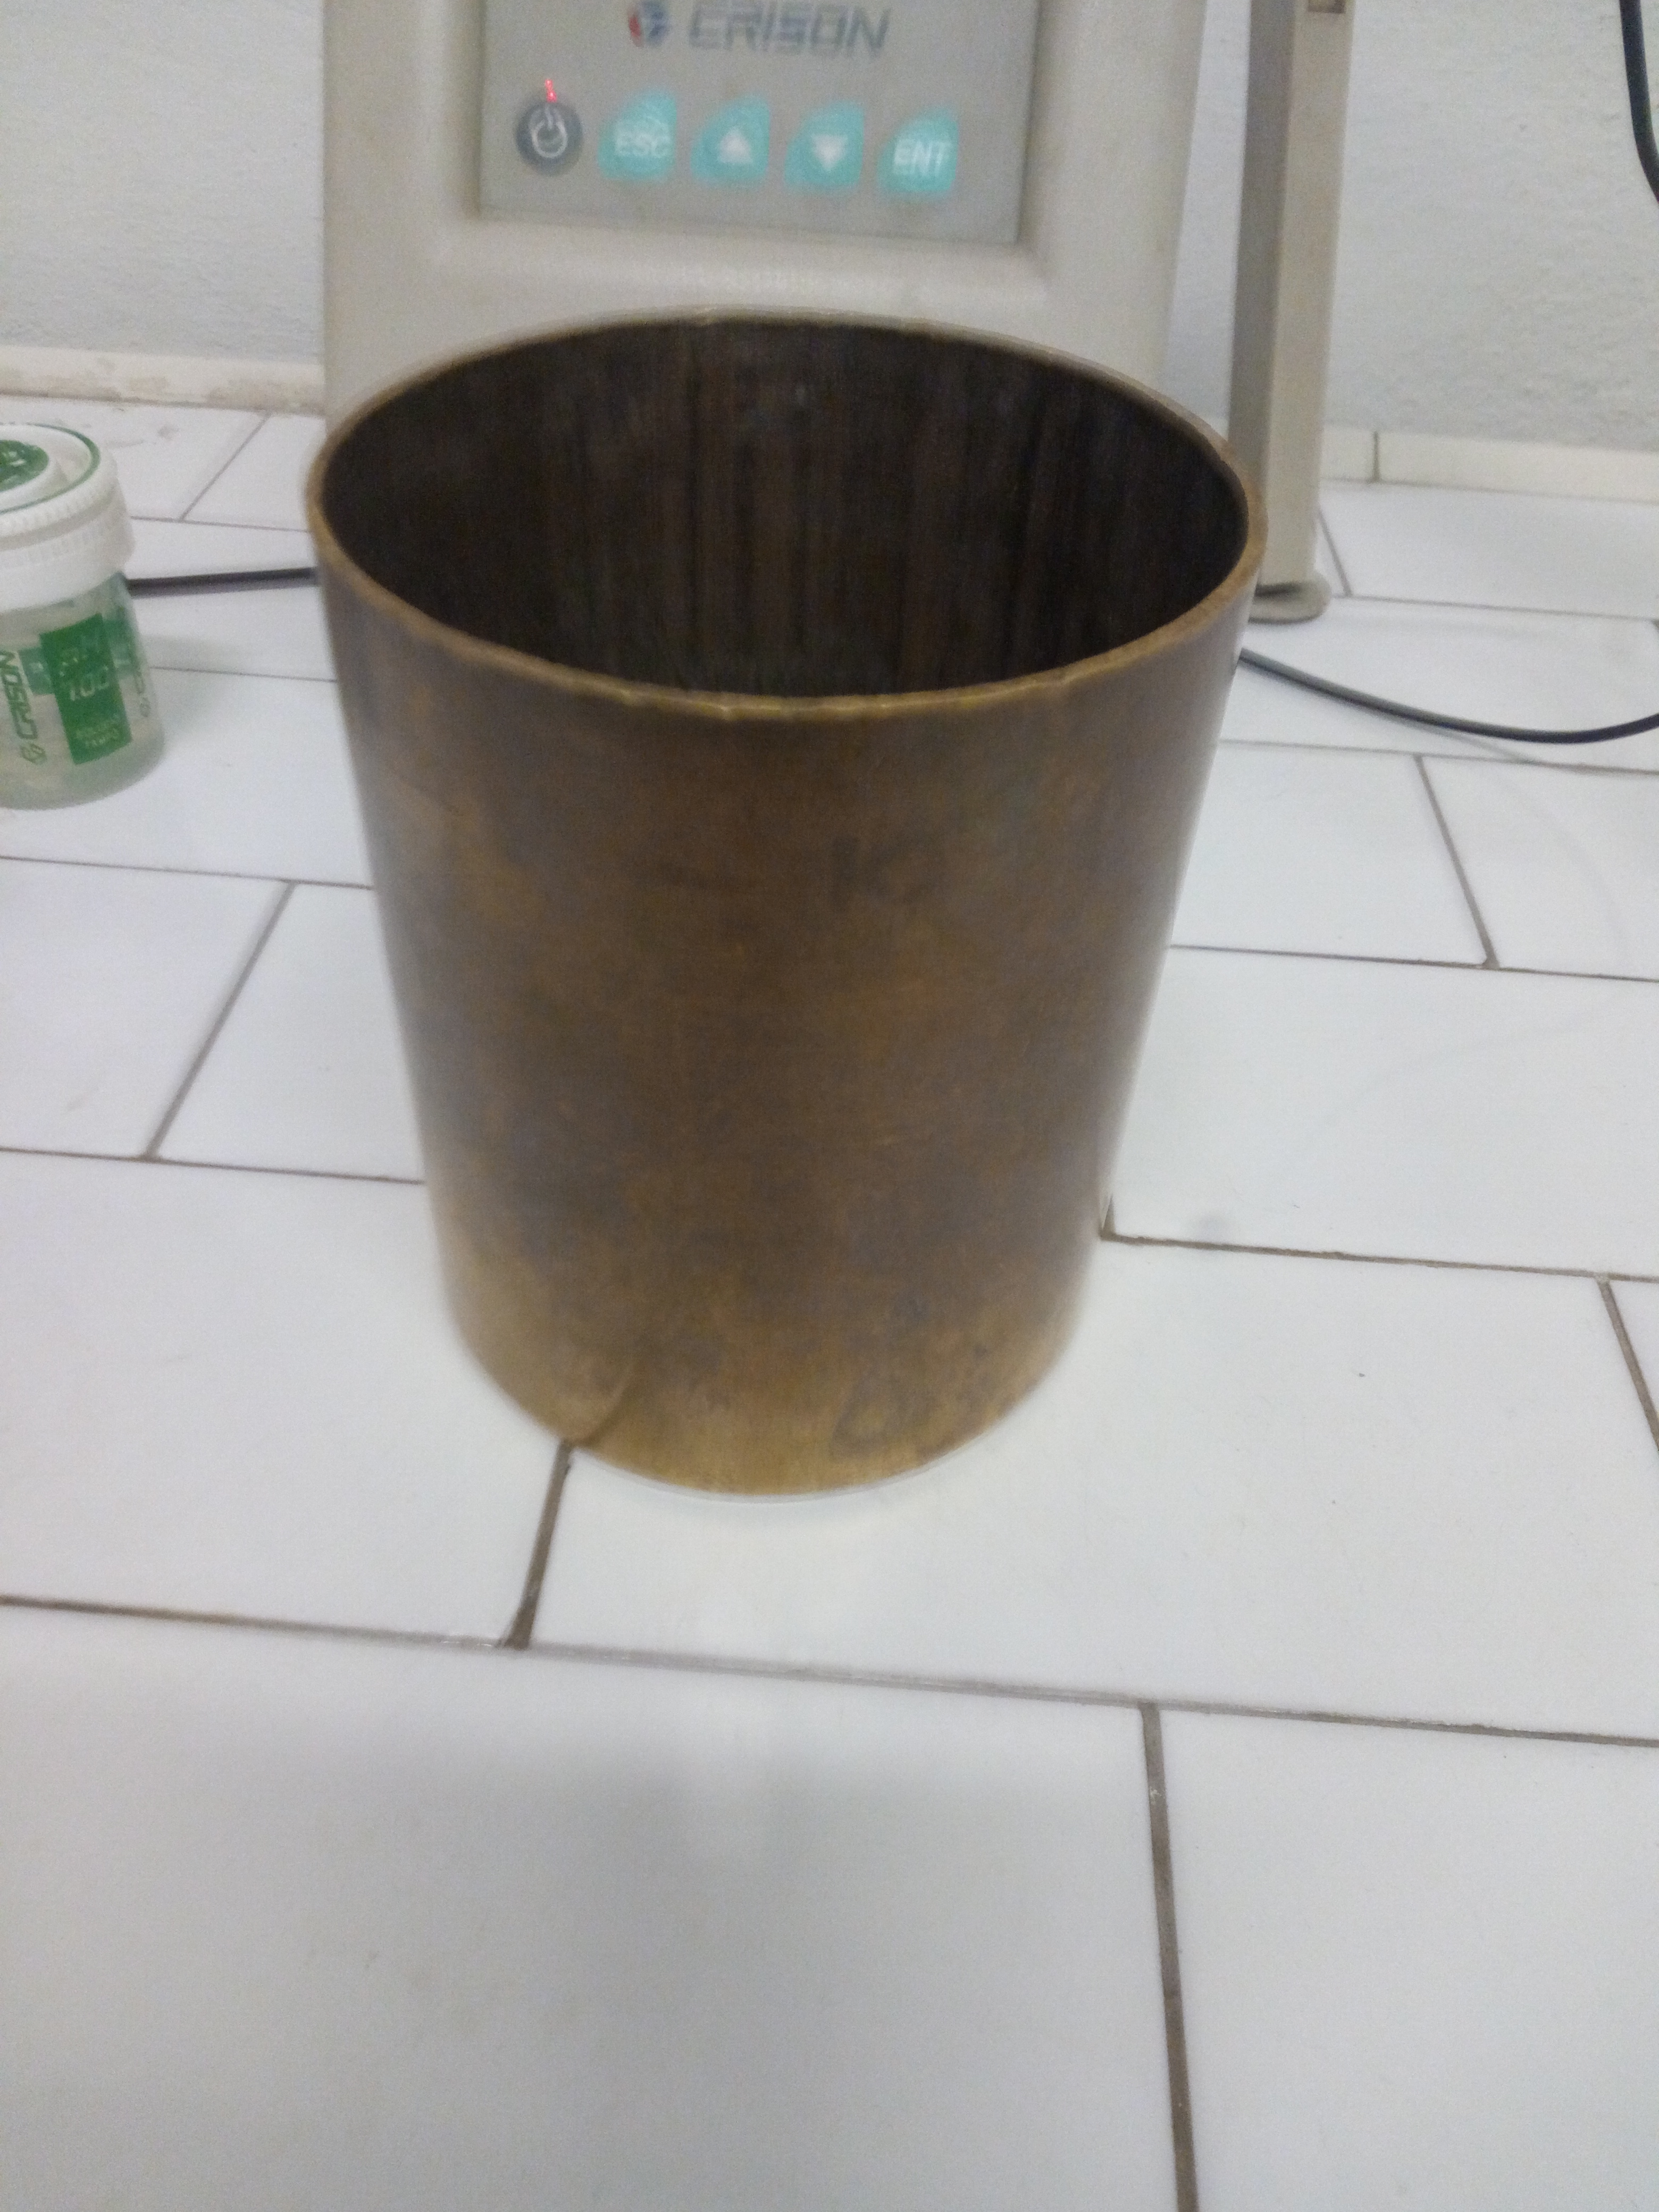
\includegraphics[width=0.8\textwidth]{../foto/cilindroOttone.jpeg}}
    \only<3>{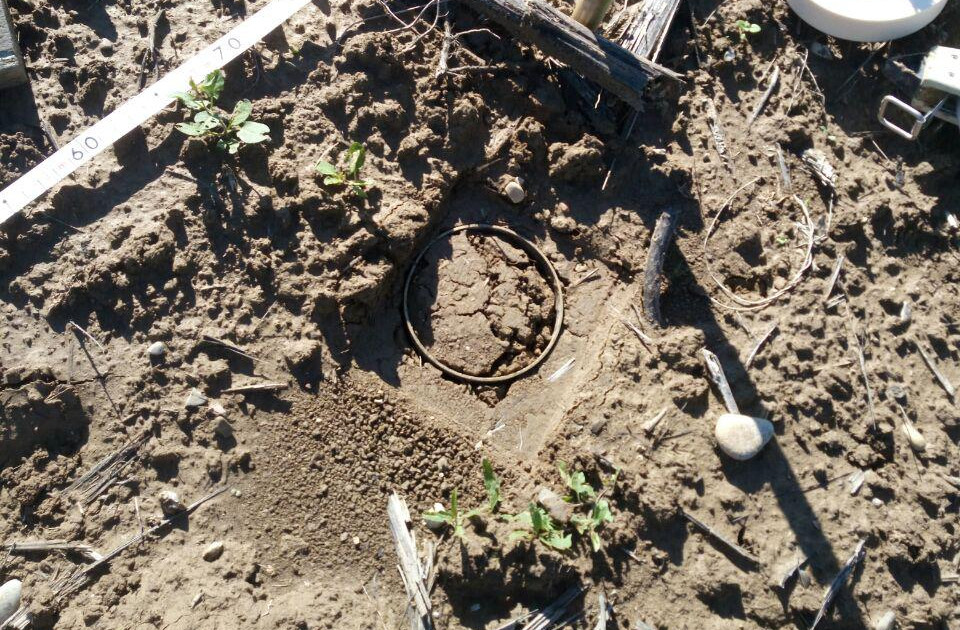
\includegraphics[width=0.8\textwidth]{../foto/cilindrosuolo.jpg}}
    \only<4>{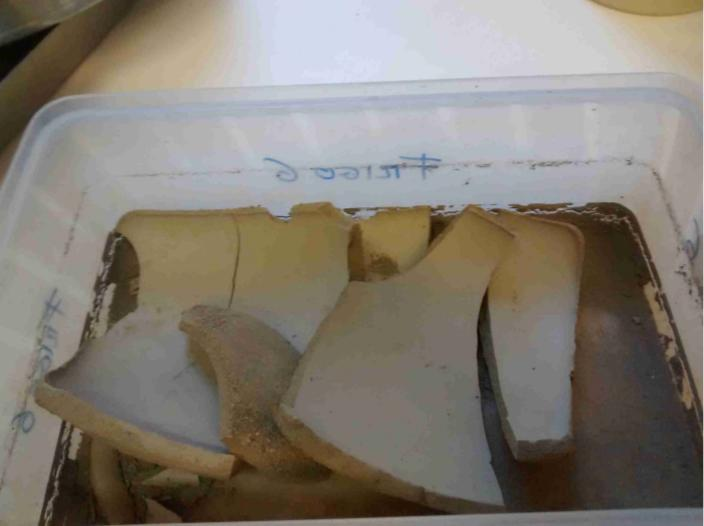
\includegraphics[width=\textwidth]{../foto/secco.jpeg}}
    \only<5>{
      \[
      \rho_{ApparenteCore} = P_{campione}/V_{cilindro}
      \]
    }
  \end{columns}
\end{frame}


\begin{frame}{Misura densita}{Due metodi: \emph{Core} e \emph{Clod}}

  \begin{columns}[c]
    \column{.50\textwidth}
    \onslide<1-> Metodo \emph{Clod}
    \pause
    \begin{itemize}[<+->]
    \item separazione di un aggregato (3-5 cm di diametro) dal
      campione di suolo
    \item misura della spinta idrostatica proporzionale, per il
      \emph{Principio di Archimede}, al volume di petrolio spostato
      dall'aggregato ($V_{aggregato}$)
    \item essiccazione a \SI{150}{\celsius} per una notte e pesatura campione
      secco ($P_{aggregato}$)
    \item calcolo della densit\`a apparente
    \end{itemize}
    \column{.48\textwidth}
    \only<2>{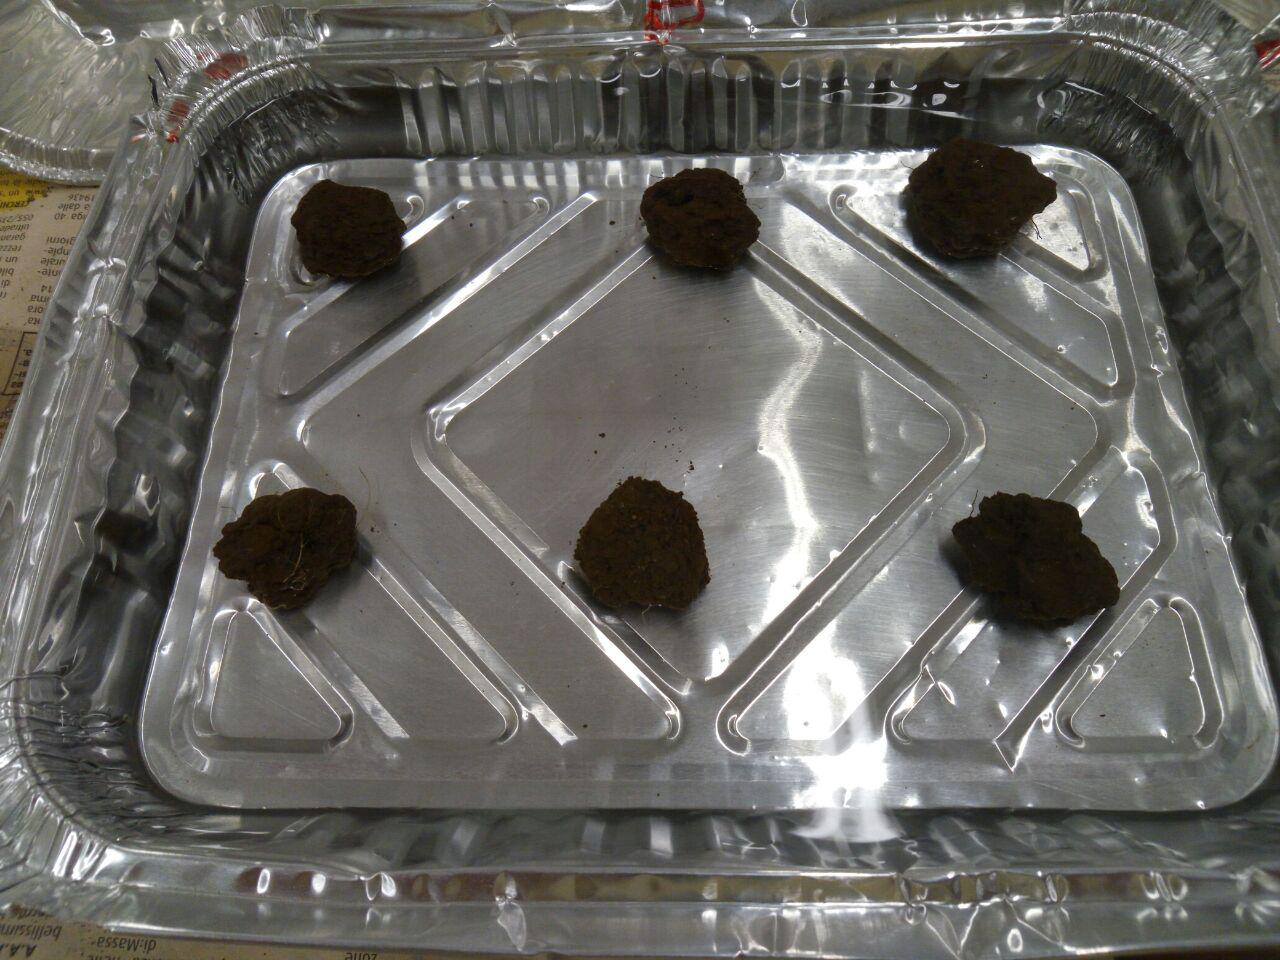
\includegraphics[width=\textwidth]{../foto/petrolio.jpeg}}
    \only<3>{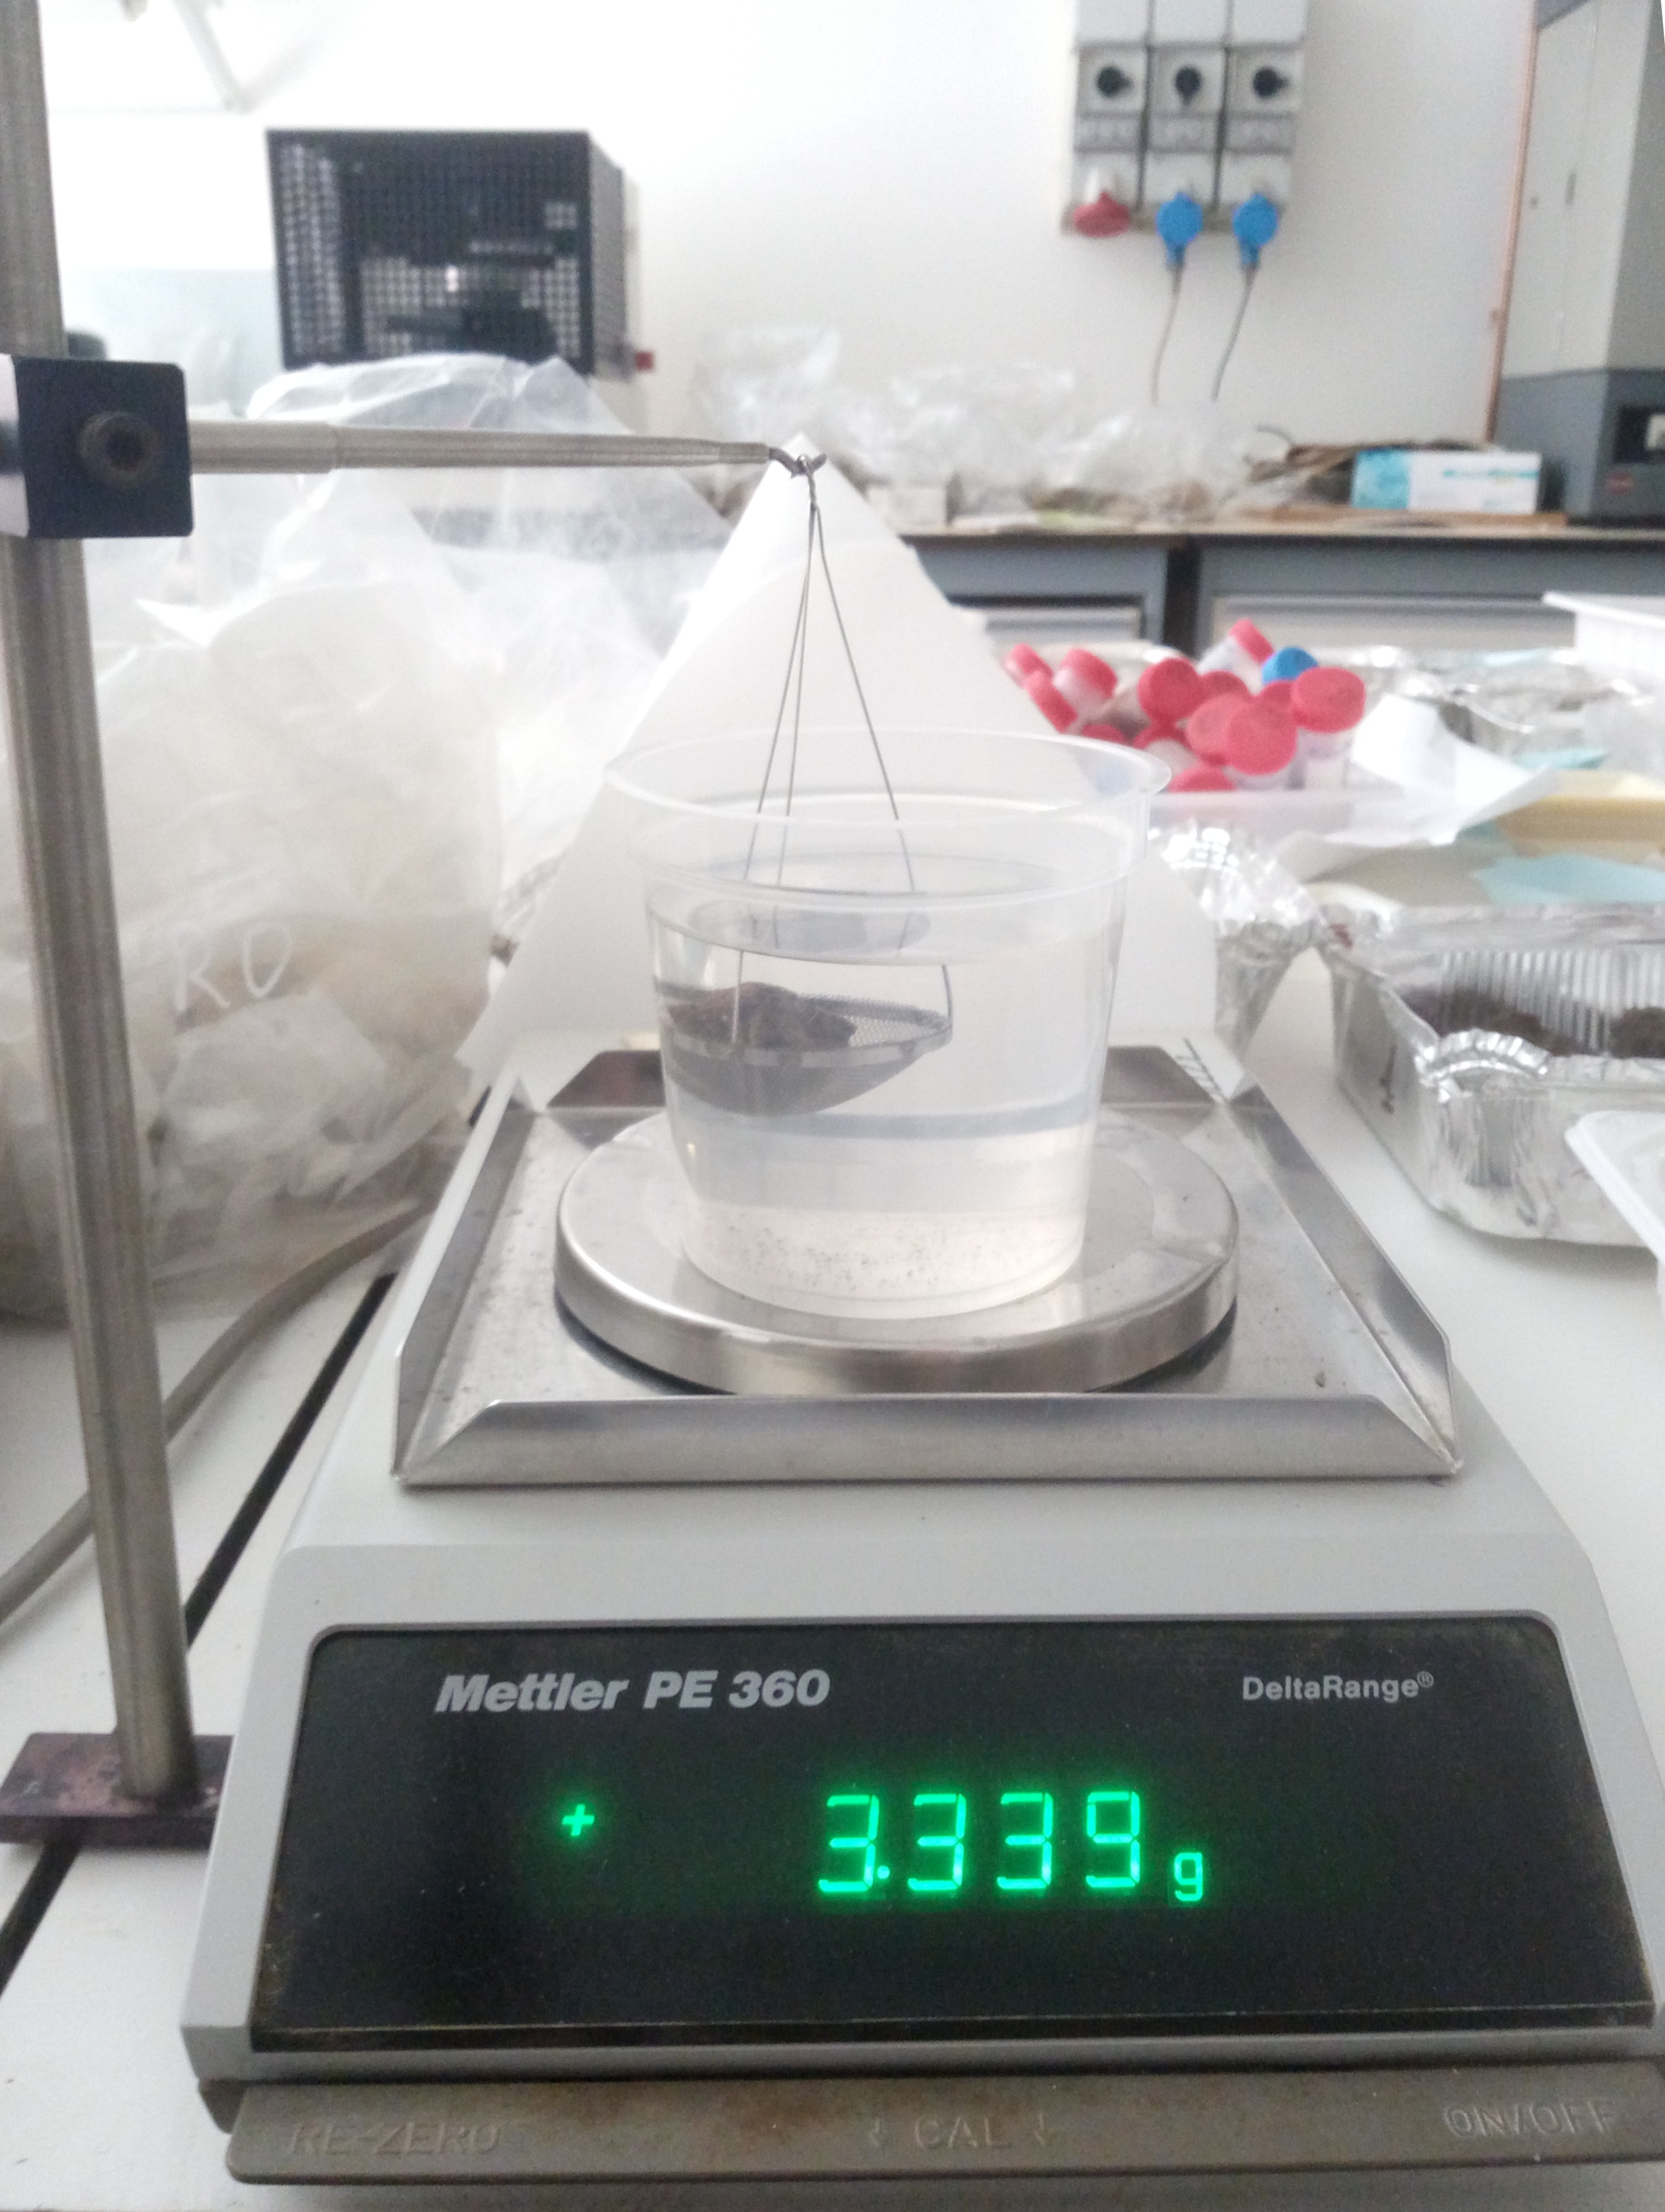
\includegraphics[width=0.8\textwidth]{../foto/navicella.jpeg}}
    \only<4>{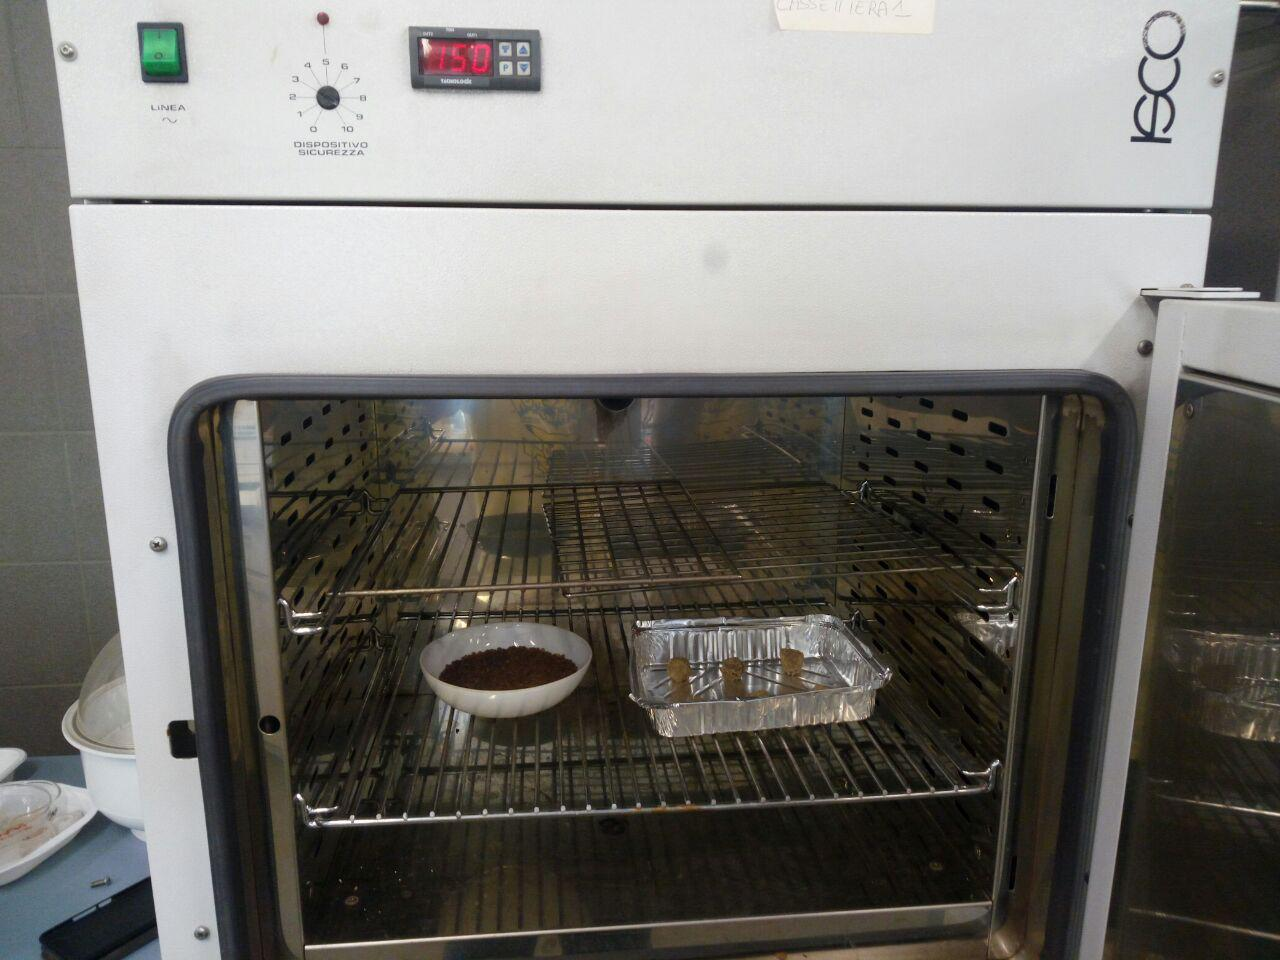
\includegraphics[width=\textwidth]{../foto/fornospinta.jpeg}}
    \only<5>{
      \[
      \rho_{ApparenteClod} = V_{aggregato}/P_{aggregato}
      \]}    
  \end{columns}

\end{frame}

\subsection{Adattamento del modello lineare}
\begin{frame}
  \frametitle{Sintesi tramite modello lineare}
  \transwipe<4>[direction=90]
  \begin{itemize}
    \onslide<1->\item 
    \vspace{0.25cm}
    $Y \sim \mu + \beta_1x_1 + \beta_2x_2 + \epsilon$
    \vspace{0.25cm}

    \onslide<2->{in cui le variabili categoriche sono:}
    \begin{itemize}

      \onslide<3->\item $\beta_1$ conduzione \newline
      \emph{Convenzionale}, \emph{Biologico}

      \onslide<4->\item $\beta_2$ lavorazioni \newline \emph{Arato, Rippato,
        Frangizollato}

      \onslide<5->\item$\epsilon$ residui o errore
    \end{itemize}
    \onslide<6->\item validazione del modello attraverso l'analisi
    dei residui 
    \onslide<7->\item analisi della varianza (ANOVA)
  \end{itemize}
\end{frame}

\subsection{Risultati}
\begin{frame}[label=densita]
  Dall'analisi statistica \`e emerso che:
  \begin{itemize}[<+->]
  \item dai dati ricavati tramite
    l'analisi col metodo \hyperlink{Core}{\beamerbutton{Core}} non sono
    state riscontrate differenze statisticamente significative tra i
    trattamenti
  \item dai dati ricavati tramite l'analisi col metodo
    \hyperlink{Clod}{\beamerbutton{Clod}} sono state riscontrate
    differenze significative tra i trattamenti tuttavia le \hyperlink{summary}{\beamerbutton{differenze}}
    sono sulla seconda cifra decimale:
    \begin{itemize}[<+->]
    \item numero di campioni adeguato
    \item differenze poco rilevanti dal punto di vista pratico
    \end{itemize}
  \end{itemize}
\end{frame}


\section{Stabilit\`a degli aggregati}
% \subsection{Strumentazione e metodo}
\begin{frame}
  \frametitle{Misura stabilit\`a degli aggregati}
  % \citep{ugolini2010basi} 
  \begin{columns}
    \column{.50\textwidth}
    % \begin{block}{}
    \pause
    \begin{enumerate}[<+->] 
    \item immissione degli aggregati di terreno setacciati nella vasca
      dello strumento
    \item acquisizione ottica della distribuzione granulometrica:
      una al minuto per 12 minuti durante i quali \ldots
    \item lo strumento provvede al ricircolo dell'acqua che disgrega
      le particelle di suolo
    \item attivazione della sonicazione dal \SI{13}{\degree} al
      \SI{24}{\degree} minuto per completare la rottura degli
      aggregati
    \end{enumerate}

    \column{.48\textwidth}
    \only<2>{
      \begin{figure}[ht]
        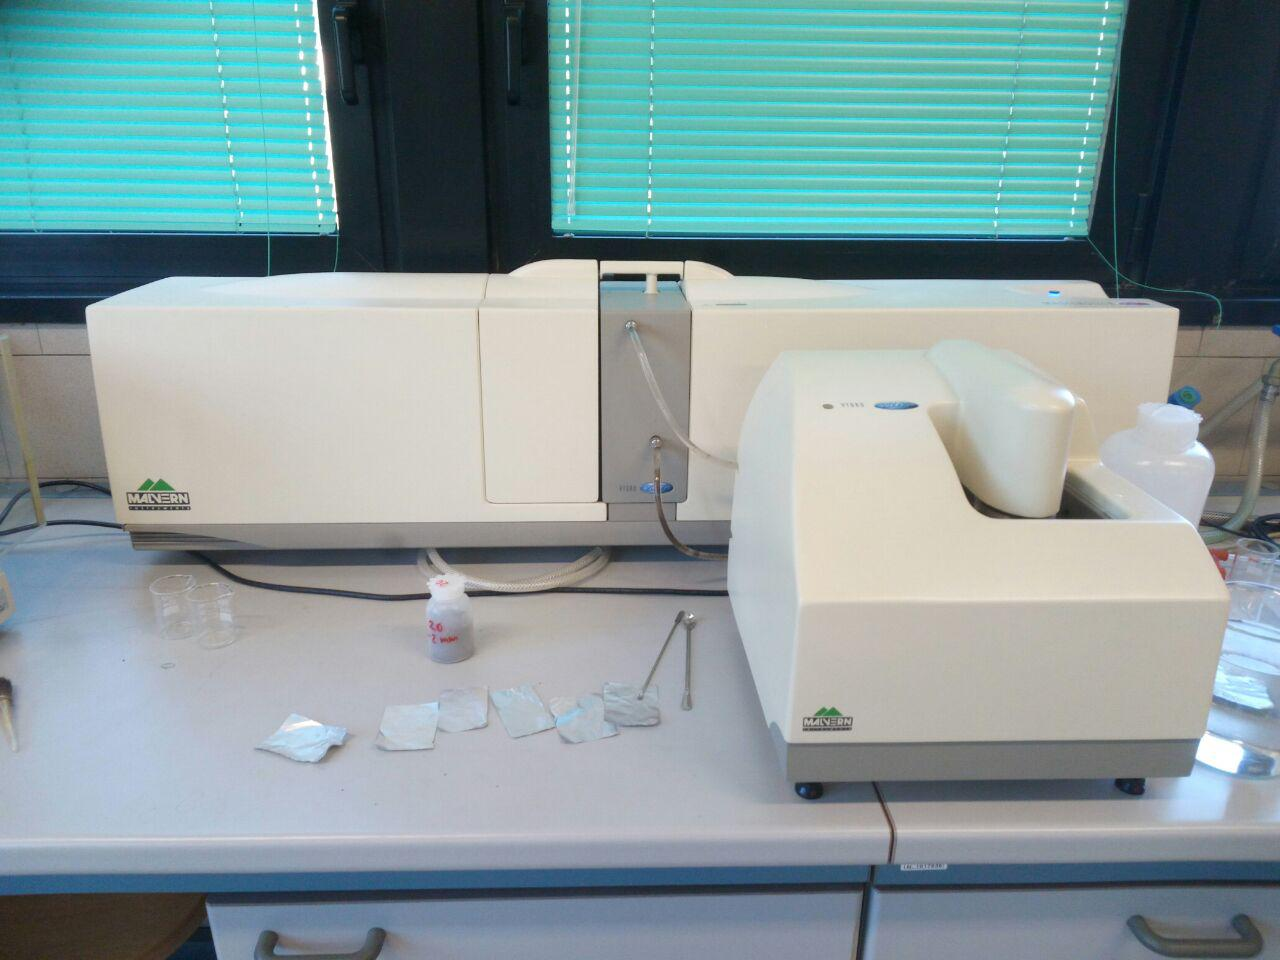
\includegraphics[width=\textwidth]{../foto/Hydro.jpeg}
      \end{figure}
    }
    \only<3-4>{
      \begin{figure}
        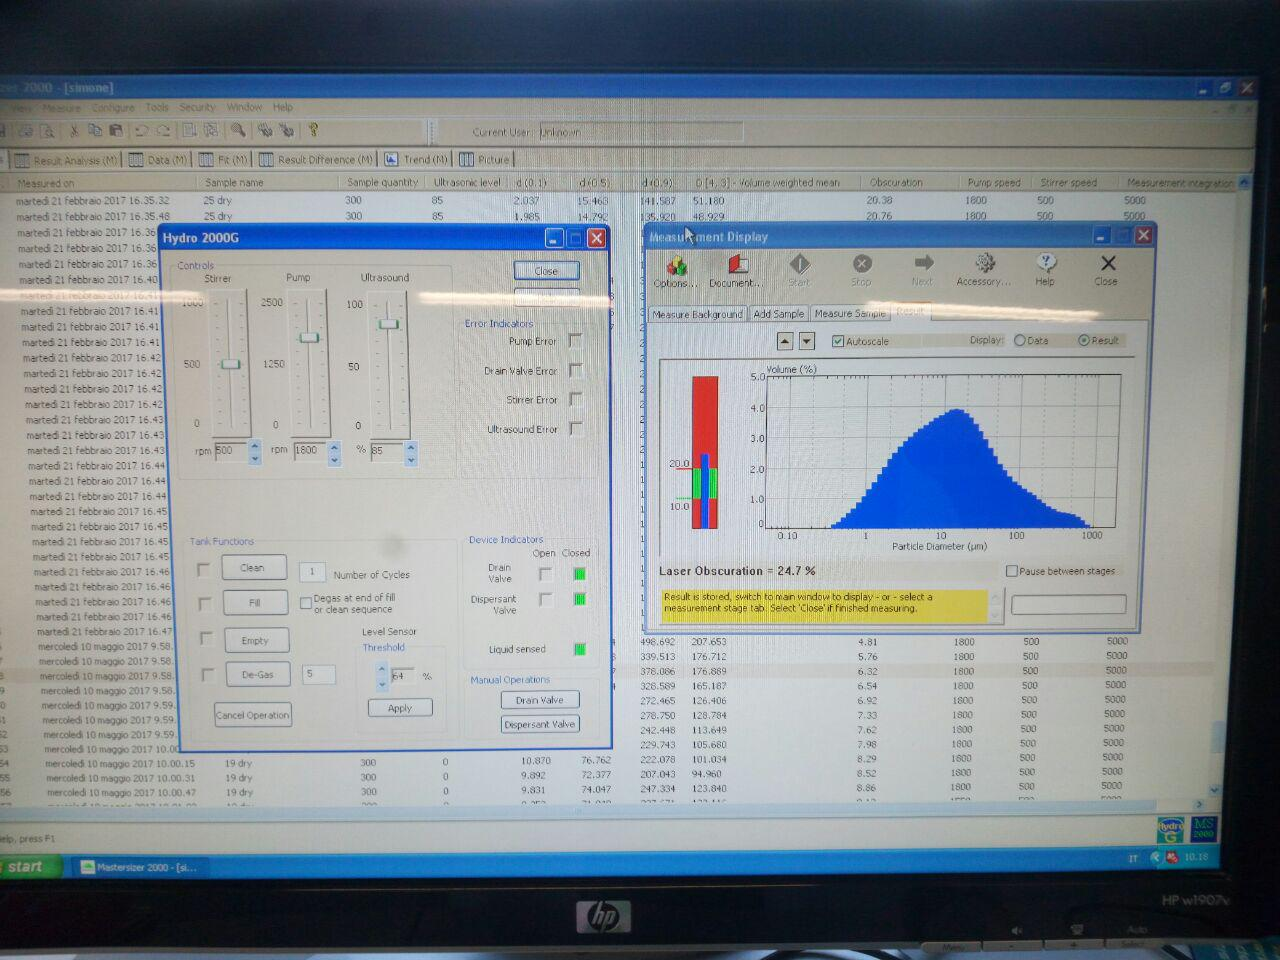
\includegraphics[width=0.8\textwidth]{../foto/Acquisiz.jpeg}
      \end{figure}
    }    
    % \only<4>{
    % \begin{figure}
    %   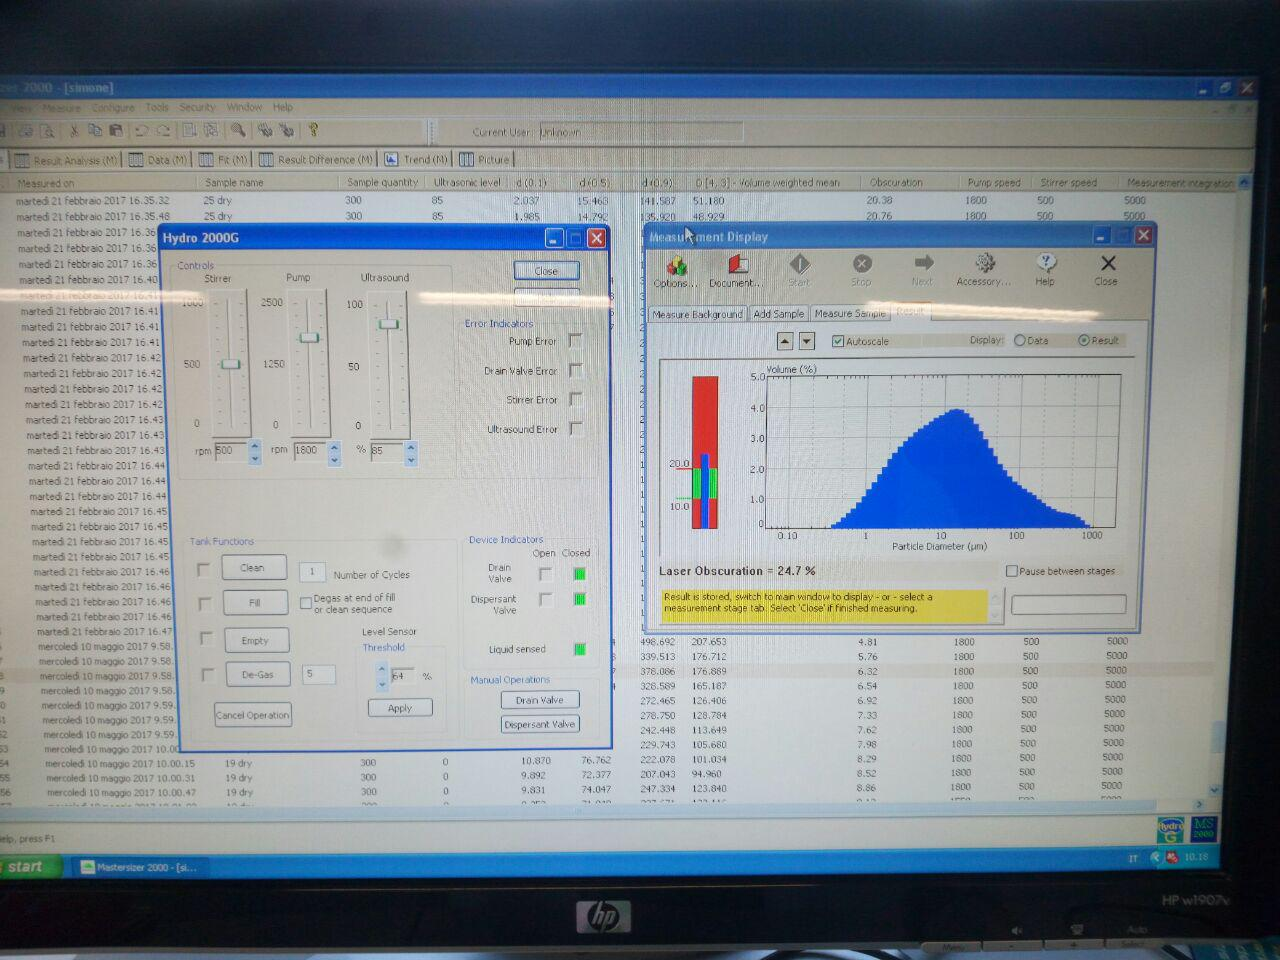
\includegraphics[width=0.8\textwidth]{../foto/Acquisiz.jpeg}
    % \end{figure}
    % } 
    \only<5>{
      \begin{figure}
        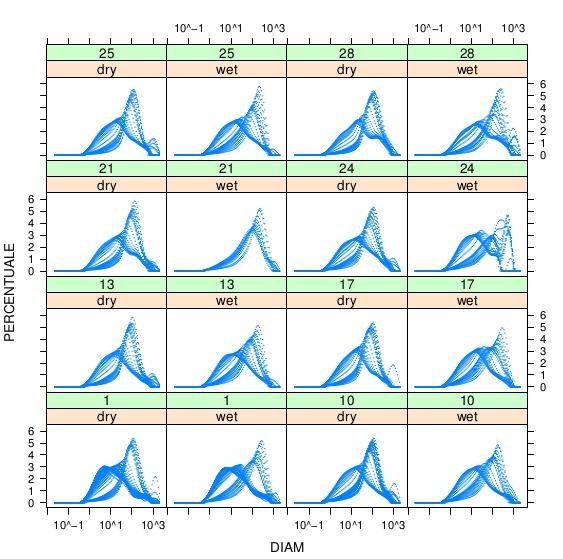
\includegraphics[width=\textwidth]{../foto/distropisa.jpeg}
      \end{figure}
    }
  \end{columns}  
\end{frame}


\begin{frame}

  \only<1>{\vspace{1.5cm}}
  \only<2>{\vspace{0.5cm}}
  \onslide<3->{\vspace{1.5cm}}
  \begin{minipage}[ht]{\textwidth}
    \footnotesize
    \begin{itemize}[<+->]
    \item i dati ottenuti sono rappresentati da distribuzioni in cui ad
      ogni classe dimensionale \`e associato il valore percentuale di
      volume sul totale
      \pause
    \item La variazione di queste distribuzioni nel tempo ci fornisce
      informazioni sulla resistenza degli aggregati alle sollecitazioni
      meccaniche.
    \item Oltre che sui campioni \textcolor{blue}{secchi}, la misura \`e
      stata ripetuta su aggregati \textcolor{magenta}{previamente
        inumiditi} per studiare la disgregazione in assenza del fenomeno
      dello \textit{slacking}
    \end{itemize}
  \end{minipage}
  \begin{minipage}[ht]{\textwidth}
    \centering
    \only<2>{
      \vspace{2cm}
      \begin{tikzpicture}[remember picture,overlay]
        \node at (current page.center) 
        {%\vspace{1cm}
          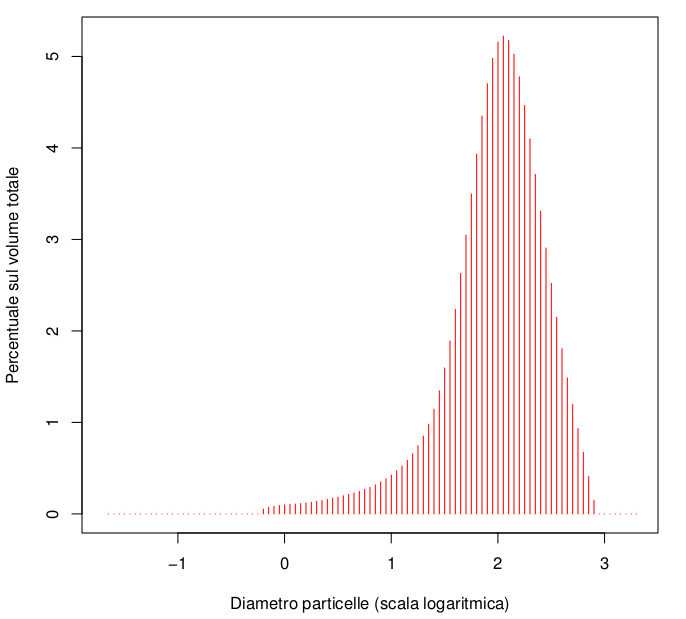
\includegraphics[width=0.5\textwidth]{../grafici/boh.jpg}
        };
      \end{tikzpicture}
      % \begin{figure}[hb][width=6cm]
      %   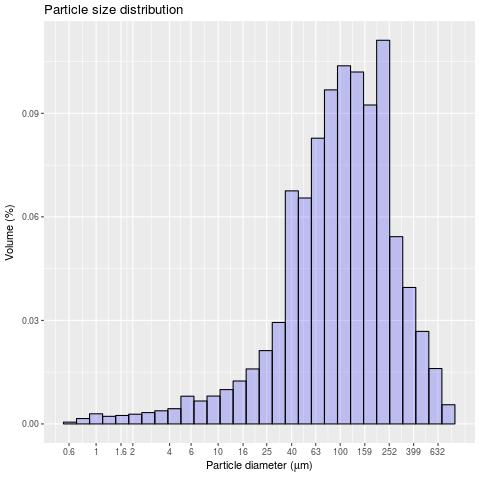
\includegraphics[width=\textwidth]{../grafici/boh.pdf}
      % \end{figure}
    }
  \end{minipage}

\end{frame}

\begin{frame}

  \vspace{1.5cm}

%  \begin{minipage}[ht]{\textwidth}
    \onslide<1->{I dati ottenuti dalla misurazione contengono porzioni di un totale,
      questo tipo di dati prende il nome di \emph{dati Composizionali}.}

    \onslide<2->{Questi sono stati elaborati tramite il package 'composition' del
      linguaggio di programmazione R}


    \onslide<3->{I dati vengono trattati tramite una \emph{Isometric
        logratio transform} che porta a definire uno spazio vettoriale
      (\emph{simplesso}) in cui possono essere applicate le tecniche di
      statistica multivariata.}
 % \end{minipage}

 % \begin{minipage}[hb]{\textwidth}
    \transdissolve<3>
 \onslide<3->{
      \begin{figure}[hb]
        \includegraphics[width=0.8\textwidth]{../foto/simplessodeforma.png}
      \end{figure}}
      % \end{minipage}
\end{frame}

\begin{frame}[label=Composizionale]
  \vspace{2cm}
  Risultati analisi \hyperlink{Anova}{\beamerbutton{composizionale}}
  \begin{figure}[hb]
    \includegraphics[width=0.6\textwidth]{../tesi/Tesi_GIT-plotacompWETDRY.pdf}
  \end{figure}
\end{frame}




% 





\section{Porosimetria}

\begin{frame}{Metodo di misura}
  \begin{columns}
    \column{.50\textwidth}
    \begin{itemize}[<+->]
    \item Separazione aggregati di circa \SI{1}{\gram}
    \item immissione degli aggregati nel \emph{dilatometro}
    \item il porosimetro riempie di mercurio il dilatometro e lo
      comprime per permetterne l'ingresso nei pori
    \item la variazione del volume di mercurio indica l'ingresso del
      mercurio nei pori 
    \item mediante l'equazione di Washburn si risale, in base alla
      pressione esercitata ($p$), al valore del diametro del poro ($r$)
    \end{itemize}
    \column{.48\textwidth}
    \only<3>{
      \begin{figure}[ht]
        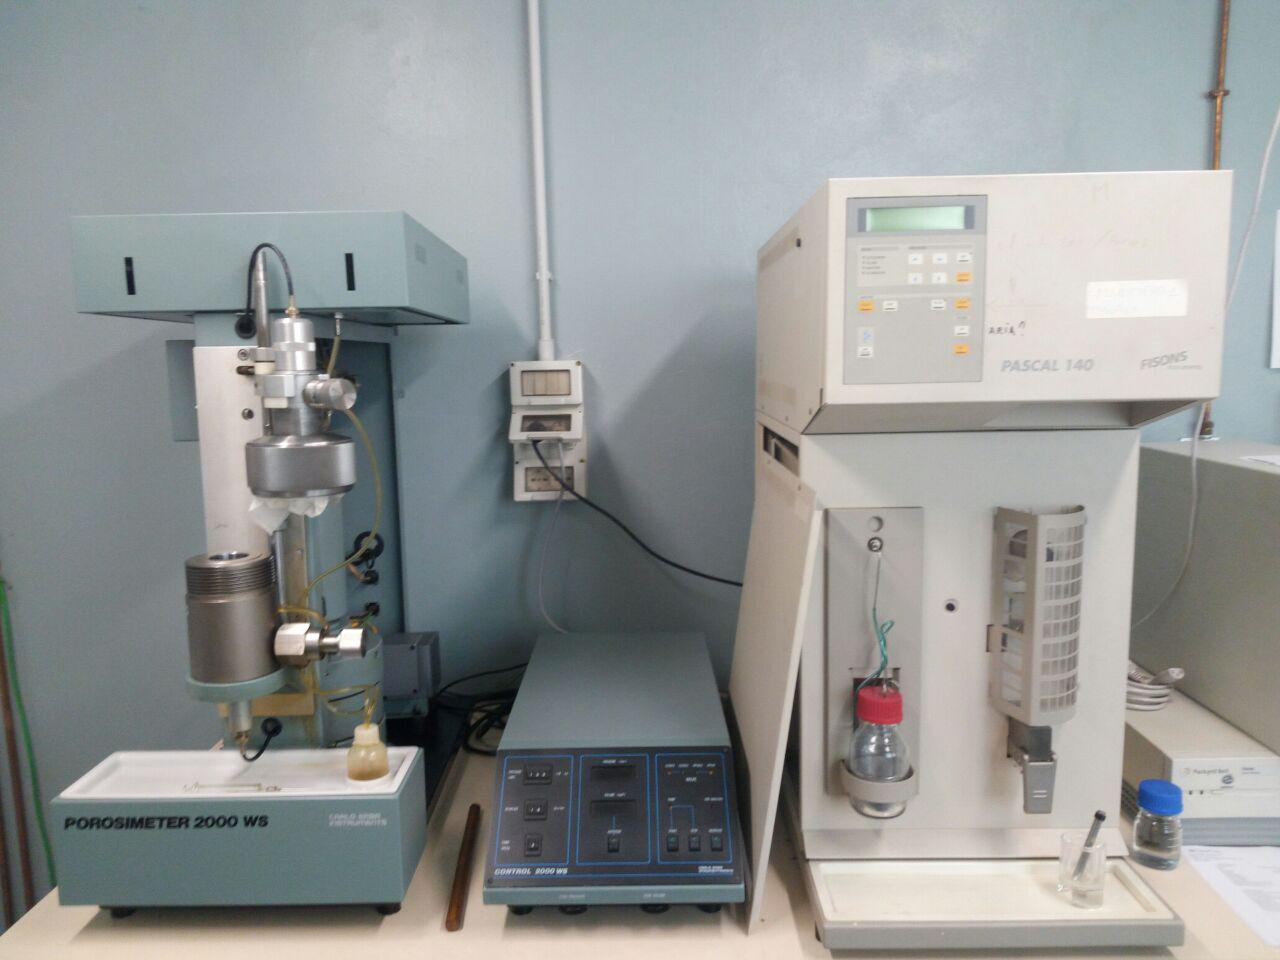
\includegraphics[width=\textwidth]{../foto/porosimetri.jpeg}
      \end{figure}
    }
\only<5>{
\large{Equazione di Washburn}

  \[
    pr=2\sigma cos \theta
    %\label{eq:Washburn}
  \]
}
  \end{columns}
\end{frame}

% \begin{frame}
%   \begin{figure}[ht]
%     \includegraphics[width=0.8\textwidth, page=8]{../grafici/penetrometria/Penetrometria2015-2016.pdf}
%   \end{figure}
% \end{frame}


% \begin{frame}
%   \begin{figure}[ht]
%     \includegraphics[width=0.8\textwidth, page=9]{../grafici/penetrometria/Penetrometria2015-2016.pdf}
%   \end{figure}
% \end{frame}

% \begin{frame}
%   \begin{figure}[ht]
%     \includegraphics[width=0.8\textwidth, page=10]{../grafici/penetrometria/Penetrometria2015-2016.pdf}
%   \end{figure}
% \end{frame}

\begin{frame}{Sintesi finale}
  \begin{itemize}[<+->]
  \item La densit\`a per grandi volumi mostra una maggior compattezza
    negli appezzamenti OO. Differenza significativa, ma solo sulla
    seconda cifra decimale. Nessun effetto delle lavorazioni
  \item La densit\`a misurata sugli aggregati mostra l'inverso (OO
    meno compatto). Anche qui differenze sulla seconda decimale. Le
    lavorazioni mostrano un effetto (aratura la pi\`u compatta)
  \item Le misure di stabilit\`a indicano un suolo generalmente poco
    stabile (aggregati inferiori a 1 mm) e che il CO produce aggregati
    di maggiori dimensioni (sia secchi che umidi).
  \item La 
  \end{itemize}

\end{frame}
\section{Porosimetria a mercurio}

\begin{frame}
  \finalpage{Boh.}
\end{frame}

%%% Local Variables:
%%% mode: latex
%%% TeX-master: t
%%% End:
\appendix
% \section{More}
% \begin{frame}[label=supplemental]
%   Supplemental content.
%   Back to .
% \end{frame}


% \subsection{Risultati Core}
\begin{frame}[label=Core]

  \vspace{1.5cm}
  \hyperlink{densita}{\beamerbutton{indietro}}
  \footnotesize
  \begin{table}[ht]
    \centering
    \begin{tabular}{lllccc}
      \hline
      Anno & Conduzione & Lavorazione & Densit\`a apparente
                                        ($g/cm^3$) & dev std & n \\ 
      \hline
      2015 & CO & Ara & 1.35 & 0.14 &   5 \\ 
           &    & Fzo & 1.34 & 0.07 &   5 \\ 
           &    & Rip & 1.38 & 0.10 &   5 \\ 
           & OO & Ara & 1.37 & 0.10 &  15 \\ 
           &    & Fzo & 1.44 & 0.10 &  15 \\ 
           &    & Rip & 1.43 & 0.07 &  15 \\ 
      \\
      2016 & CO & Ara & 1.38 & 0.16 &   6 \\ 
           &    & Fzo & 1.35 & 0.15 &   6 \\ 
           &    & Rip & 1.26 & 0.09 &   5 \\ 
           & OO & Ara & 1.37 & 0.06 &   6 \\ 
           &    & Fzo & 1.35 & 0.07 &   6 \\ 
           &    & Rip & 1.40 & 0.15 &   6 \\ 
      \hline
    \end{tabular}
    \label{tab:RiassuntoDensitaCAmpo}
  \end{table}
\end{frame}


\begin{frame}
  \vspace{1.5cm}
  \begin{figure}
    \includegraphics[width=0.8\textwidth]{../tesi/Tesi_GIT-figboh2.pdf}
  \end{figure}
\end{frame}

\begin{frame}{Tabella ANOVA per i valori di densità rilevati col metodo \emph{Core}} 
  % latex table generated in R 3.4.0 by xtable 1.8-2 package
  % Thu Jun 22 16:16:27 2017
  \begin{table}[ht]
    \centering
    \label{tab:anova del modello}
    \begin{tabular}{lrrrrr}
      \hline
      & Df & Sum Sq & Mean Sq & F value & Pr($>$F) \\ 
      \hline
      Anno & 1 & 0.02 & 0.02 & 1.41 & 0.2390 \\ 
      Conduzione & 1 & 0.04 & 0.04 & 3.29 & 0.0745 \\ 
      Lavorazione & 2 & 0.00 & 0.00 & 0.03 & 0.9728 \\ 
      Residui & 90 & 0.97 & 0.01 &  &  \\ 
      \hline
    \end{tabular}
  \end{table}
\end{frame}


\begin{frame}[label=Clod]
  \hyperlink{densita}{\beamerbutton{indietro}}
  \footnotesize
  \begin{table}[ht]
    \centering
    \begin{tabular}{llrccc}
      \hline
      Conduzione & Lavorazione & Media & Dev. std & n & Tukey \\ 
      \hline
      Convenzionale & Arato & 1.93 & 0.06 &  18 & b \\ 
                 & Frangizollato & 1.89 & 0.05 &  18 & ab \\ 
                 & Rippato & 1.90 & 0.06 &  18 & ab \\ 
      Organico & Arato & 1.90 & 0.07 &  18 & ab \\ 
                 & Frangizollato & 1.84 & 0.06 &  18 & a \\ 
                 & Rippato & 1.87 & 0.07 &  18 & ab \\ 
      \hline
    \end{tabular}
    \label{tab:RiassuntoDensitaSpinta}
  \end{table}
\end{frame}

\begin{frame}
  \vspace{1.5cm}
  \begin{figure}
    \includegraphics[width=0.8\textwidth]{../tesi/Tesi_GIT-figmah.pdf}
  \end{figure}
\end{frame}


\begin{frame}{Tabella ANOVA per i valori di densità rilevati col metodo \emph{Clod}}
  % latex table generated in R 3.4.0 by xtable 1.8-2 package
  % Thu Jun 22 16:32:35 2017
  \begin{table}
    \centering
    \begin{tabular}{llcccc}
      \hline
      & Df & Sum Sq & Mean Sq & F value & Pr($>$F) \\ 
      \hline
      Conduzione & 1 & 0.03 & 0.03 & 6.31 & 0.012 \\ 
      Lavorazione & 2 & 0.05 & 0.02 & 5.83 & 0.004 \\ 
      Totale & 104 & 0.42 & 0.00 &  &  \\ 
      \hline
    \end{tabular}
    \label{tab:Anova densita per spinta}
  \end{table}
\end{frame}

\begin{frame}[label=summary]
  % \hyperlink{densita}{\beamerbutton{indietro}}
  % latex table generated in R 3.4.0 by xtable 1.8-2 package
  % Thu Jun 22 10:44:00 2017
  \footnotesize
  % latex table generated in R 3.4.0 by xtable 1.8-2 package
  % Thu Jun 22 16:31:31 2017
  \begin{table}[ht]
    \centering
    \begin{tabular}{rrrrr}
      \hline
      & Estimate & Std. Error & t value & Pr($>$$|$t$|$) \\ 
      \hline
      % Convenzionale arato & 1.9470 & 0.0295 & 65.98 & 0.0000 \\ 
      % Scostamento biologico & -0.0534 & 0.0295 & -1.81 & 0.0731 \\ 
      % Scostamento frangizollato & -0.0780 & 0.0361 & -2.16 & 0.0331 \\ 
      % Scostamento rippato & -0.0881 & 0.0361 & -2.44 & 0.0164 \\ 
      Convenzionale arato & 1.93 & 0.01 & 157.38 & 0.000 \\ 
      Scostamento biologico & -0.03 & 0.01 & -2.51 & 0.014 \\ 
      Scostamento frangizollato & -0.05 & 0.02 & -3.39 & 0.001 \\ 
      Scostamento rippato & -0.03 & 0.02 & -2.04 & 0.043 \\ 
      \hline
    \end{tabular}
    \label{tab:Riassunto densita spinta}
  \end{table}
\end{frame}

\begin{frame}[label=Anova]
  \hyperlink{Composizionale}{\beamerbutton{indietro}}
  \footnotesize
  % latex table generated in R 3.4.0 by xtable 1.8-2 package
  % Tue Jun 27 21:29:19 2017
  \begin{table}
    \centering
    \begin{tabular}{lrrrrcr}
      \hline
      & Df & Pillai & approx F & num Df & den Df & Pr($>$F) \\ 
      \hline
      Convenzionale & 1 & 0.92 & 4955.26 & 2 & 835 & $<10^{-3}$ \\ 
      Biologico  & 1 & 0.09 & 41.72 & 2 & 835 &  $<10^{-3}$ \\ 
      Tempo & 1 & 0.92 & 4504.77 & 2 & 835 &  $<10^{-3}$  \\ 
      Tempo$^2$& 1 & 0.35 & 227.06 & 2 & 835 &  $<10^{-3}$ \\ 
      Totale & 836 &  &  &  &  &  \\ 
      \hline
    \end{tabular}
  \end{table}
\end{frame}


\end{document}
